\documentclass[17pt]{extarticle}
\usepackage{tikz}
\usepackage{pgfmath,pgffor}
\begin{document}
\def\names{{"blue","brown","cyan","darkgray",
            "gray","green","lime","magenta",
            "olive","orange","pink","purple",
            "red","teal","violet","yellow"}}%
% \foreach \i in {0,...,15} {%
% \pgfmathparse{\names[\i]}\pgfmathresult, }

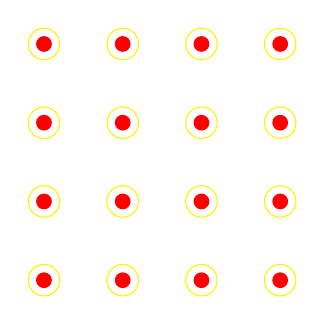
\begin{tikzpicture}
  \foreach \x in {0,1,2,3}
    \foreach \y in {0,1,2,3}
      {
        \draw [color=yellow] (\x,\y) circle (0.2cm);
        \fill [red](\x,\y) circle (0.1cm);
      }
\end{tikzpicture}


\end{document}
\end{document}
